\documentclass[11pt]{article}
\usepackage[textwidth=18.0cm, textheight=23.0cm, top=2.0cm]{geometry}
\usepackage{pst-all}
\usepackage{amssymb}
\usepackage{tikz}
\usepackage{underscore}\begin{document}
\pagestyle{empty}


ClassName: \underline{\textbf{Class_03.2bp-28}}
\par
BinSize: \underline{\textbf{40 × 40}}
\par
ReduceSize: \underline{\textbf{40 × 40}}
\par
TypeNum: \underline{\textbf{59}}
\par
Num: \underline{\textbf{60}}
\par
OutS: \underline{\textbf{20800}}
\par
InS: \underline{\textbf{18511}}
\par
Rate: \underline{\textbf{0.890}}
\par
UB: \underline{\textbf{13}}
\par
LB0: \underline{\textbf{13}}
\par
LB: \underline{\textbf{13}}
\par
LBWithCut: \underline{\textbf{13}}
\par
NodeCut: \underline{\textbf{0}}
\par
ExtendedNodeCnt: \underline{\textbf{1}}
\par
GenNodeCnt: \underline{\textbf{1}}
\par
PrimalNode: \underline{\textbf{0}}
\par
ColumnCount: \underline{\textbf{13}}
\par
TotalCutCount: \underline{\textbf{0}}
\par
RootCutCount: \underline{\textbf{0}}
\par
LPSolverCnt: \underline{\textbf{1}}
\par
PricingSolverCnt: \underline{\textbf{0}}
\par
BranchAndBoundNum: \underline{\textbf{1}}
\par
isOpt: \underline{\textbf{true}}
\par
TimeOnInitSolution: \underline{\textbf{600.000 s}}
\par
TimeOnPrimal: \underline{\textbf{0.000 s}}
\par
TimeOnPricing: \underline{\textbf{0.000 s}}
\par
TimeOnRmp: \underline{\textbf{0.079 s}}
\par
TotalTime: \underline{\textbf{600.344 s}}
\par
\newpage


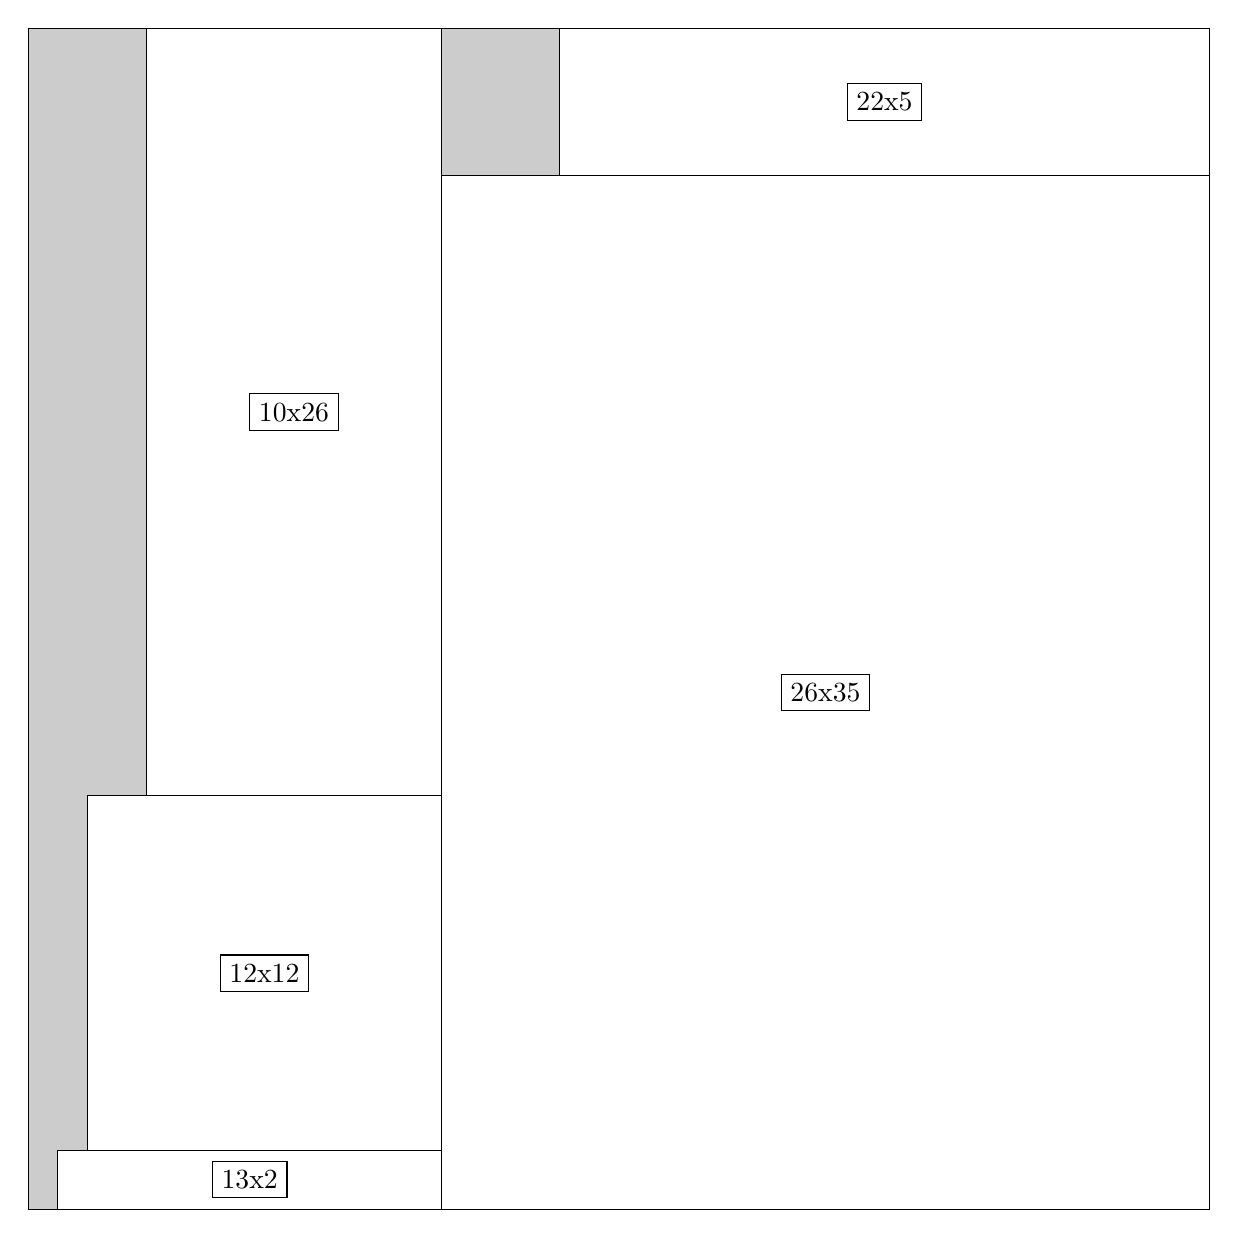
\begin{tikzpicture}[shorten >=1pt,scale=1.0,every node/.style={scale=1.0},->]
\tikzstyle{vertex}=[circle,fill=black!25,minimum size=14pt,inner sep=0pt]
\filldraw[fill=gray!40!white, draw=black] (0,0) rectangle (15.0,15.0);
\foreach \name/\x/\y/\w/\h in {26x35/5.25/0.0/9.75/13.125,22x5/6.75/13.125/8.25/1.875,13x2/0.375/0.0/4.875/0.75,12x12/0.75/0.75/4.5/4.5,10x26/1.5/5.25/3.75/9.75}
\filldraw[fill=white!40!white, draw=black] (\x,\y) rectangle node[draw] (\name) {\name} ++(\w,\h);
\end{tikzpicture}


w =26 , h =35 , x =14 , y =0 , v =910
\par
w =22 , h =5 , x =18 , y =35 , v =110
\par
w =13 , h =2 , x =1 , y =0 , v =26
\par
w =12 , h =12 , x =2 , y =2 , v =144
\par
w =10 , h =26 , x =4 , y =14 , v =260
\par
\newpage


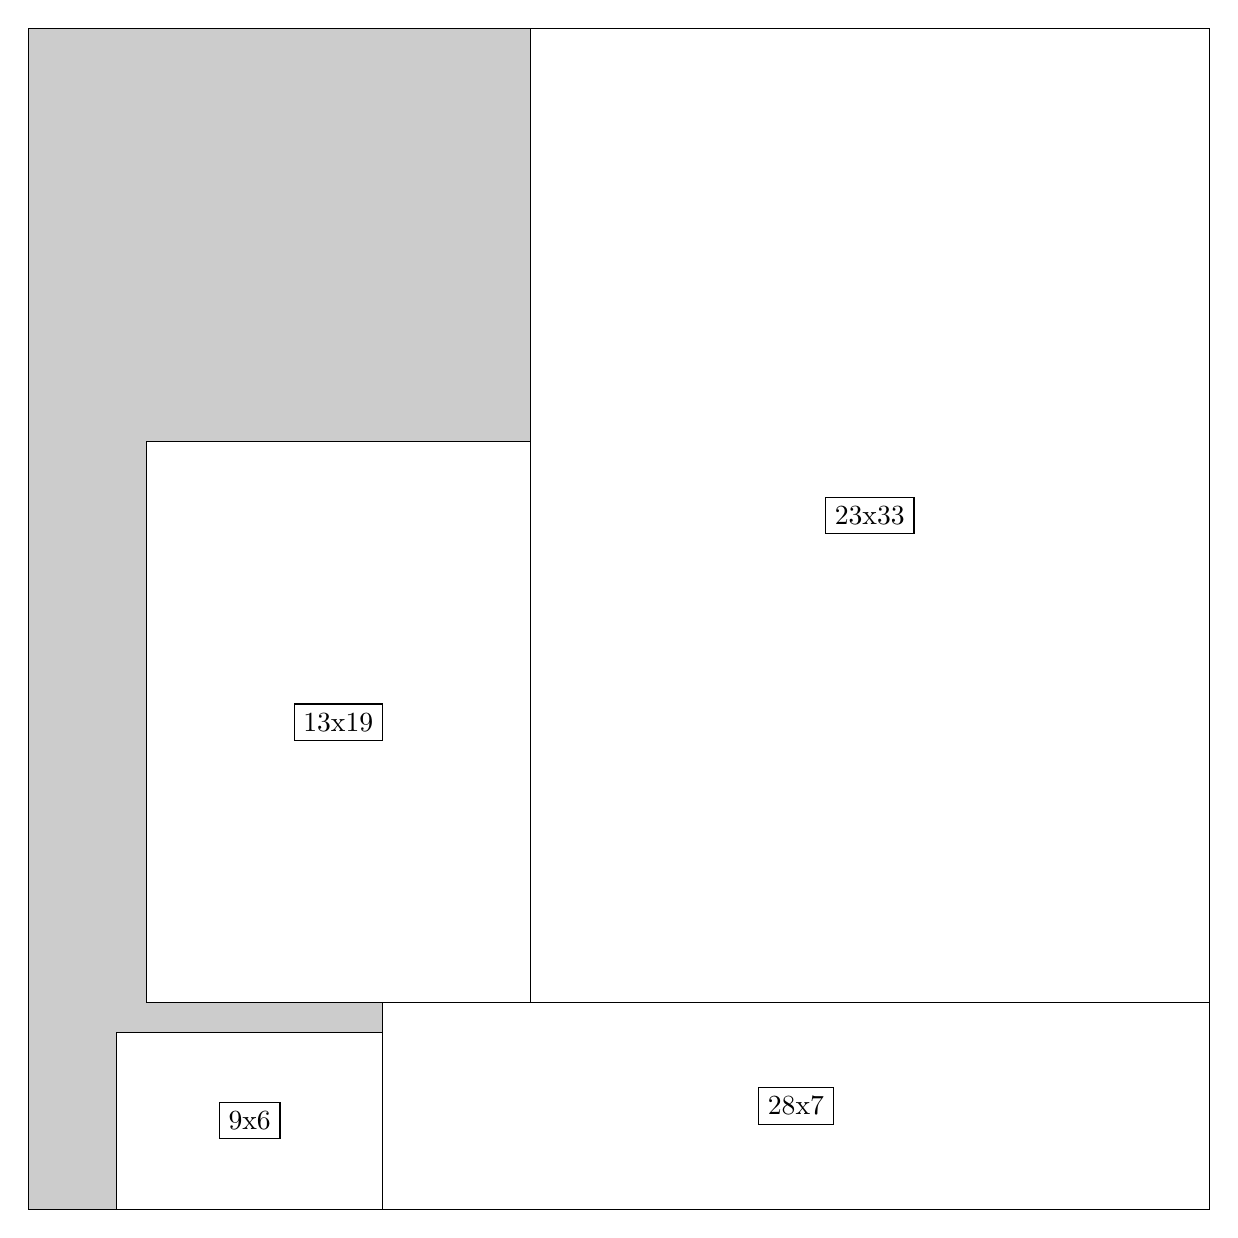
\begin{tikzpicture}[shorten >=1pt,scale=1.0,every node/.style={scale=1.0},->]
\tikzstyle{vertex}=[circle,fill=black!25,minimum size=14pt,inner sep=0pt]
\filldraw[fill=gray!40!white, draw=black] (0,0) rectangle (15.0,15.0);
\foreach \name/\x/\y/\w/\h in {28x7/4.5/0.0/10.5/2.625,9x6/1.125/0.0/3.375/2.25,23x33/6.375/2.625/8.625/12.375,13x19/1.5/2.625/4.875/7.125}
\filldraw[fill=white!40!white, draw=black] (\x,\y) rectangle node[draw] (\name) {\name} ++(\w,\h);
\end{tikzpicture}


w =28 , h =7 , x =12 , y =0 , v =196
\par
w =9 , h =6 , x =3 , y =0 , v =54
\par
w =23 , h =33 , x =17 , y =7 , v =759
\par
w =13 , h =19 , x =4 , y =7 , v =247
\par
\newpage


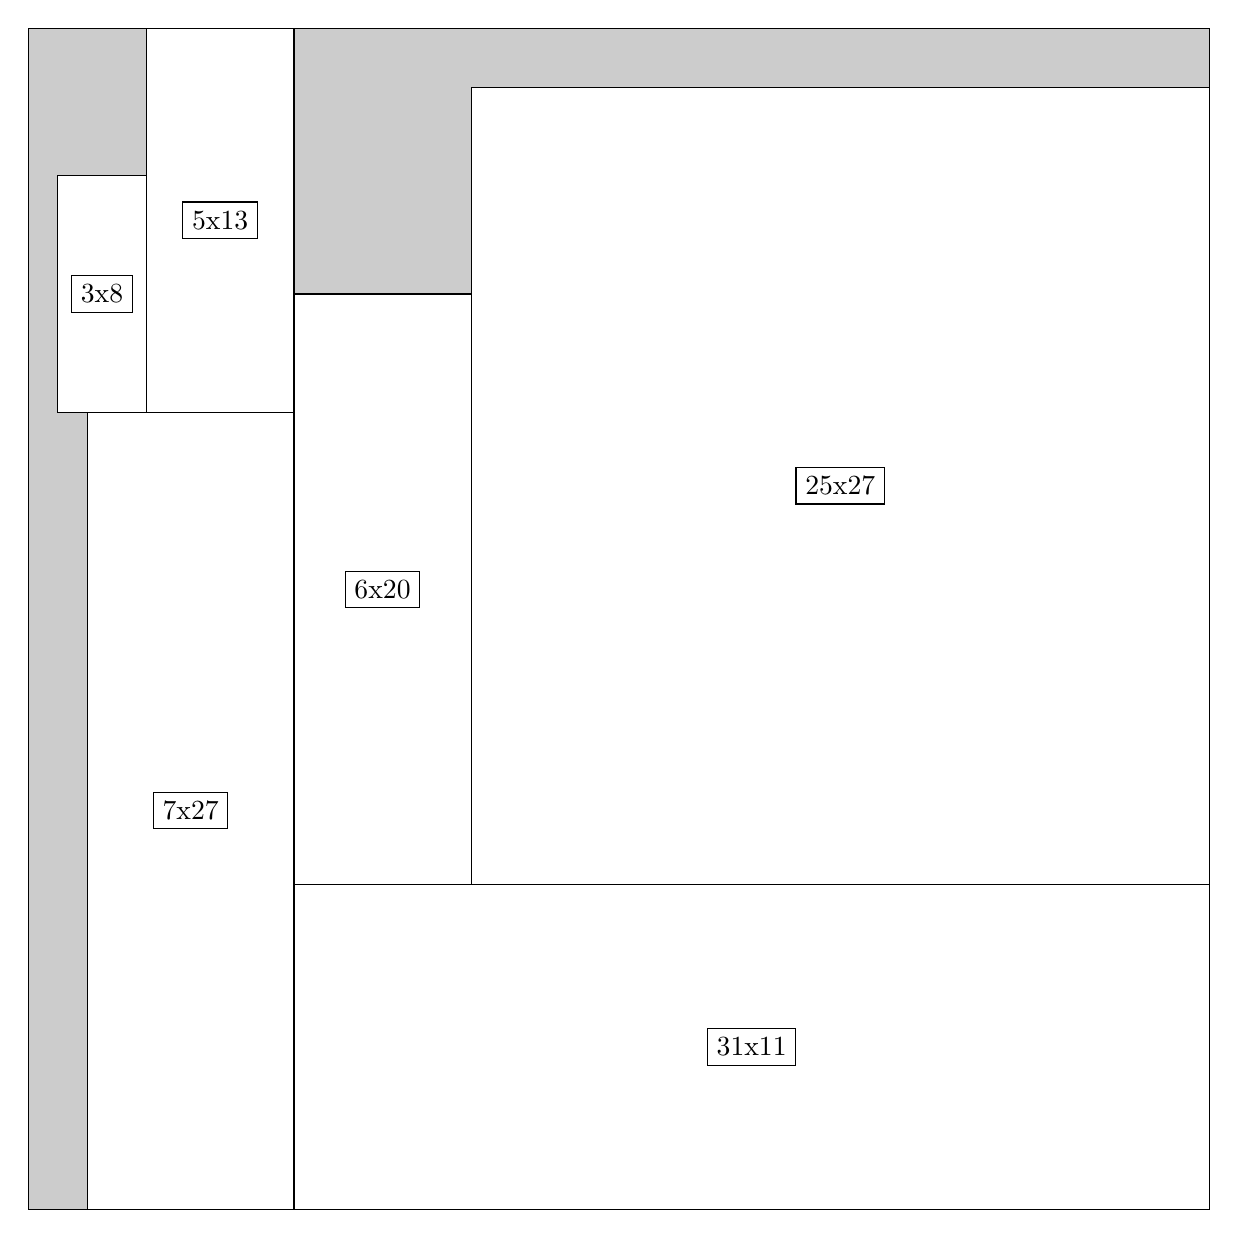
\begin{tikzpicture}[shorten >=1pt,scale=1.0,every node/.style={scale=1.0},->]
\tikzstyle{vertex}=[circle,fill=black!25,minimum size=14pt,inner sep=0pt]
\filldraw[fill=gray!40!white, draw=black] (0,0) rectangle (15.0,15.0);
\foreach \name/\x/\y/\w/\h in {31x11/3.375/0.0/11.625/4.125,25x27/5.625/4.125/9.375/10.125,6x20/3.375/4.125/2.25/7.5,7x27/0.75/0.0/2.625/10.125,5x13/1.5/10.125/1.875/4.875,3x8/0.375/10.125/1.125/3.0}
\filldraw[fill=white!40!white, draw=black] (\x,\y) rectangle node[draw] (\name) {\name} ++(\w,\h);
\end{tikzpicture}


w =31 , h =11 , x =9 , y =0 , v =341
\par
w =25 , h =27 , x =15 , y =11 , v =675
\par
w =6 , h =20 , x =9 , y =11 , v =120
\par
w =7 , h =27 , x =2 , y =0 , v =189
\par
w =5 , h =13 , x =4 , y =27 , v =65
\par
w =3 , h =8 , x =1 , y =27 , v =24
\par
\newpage


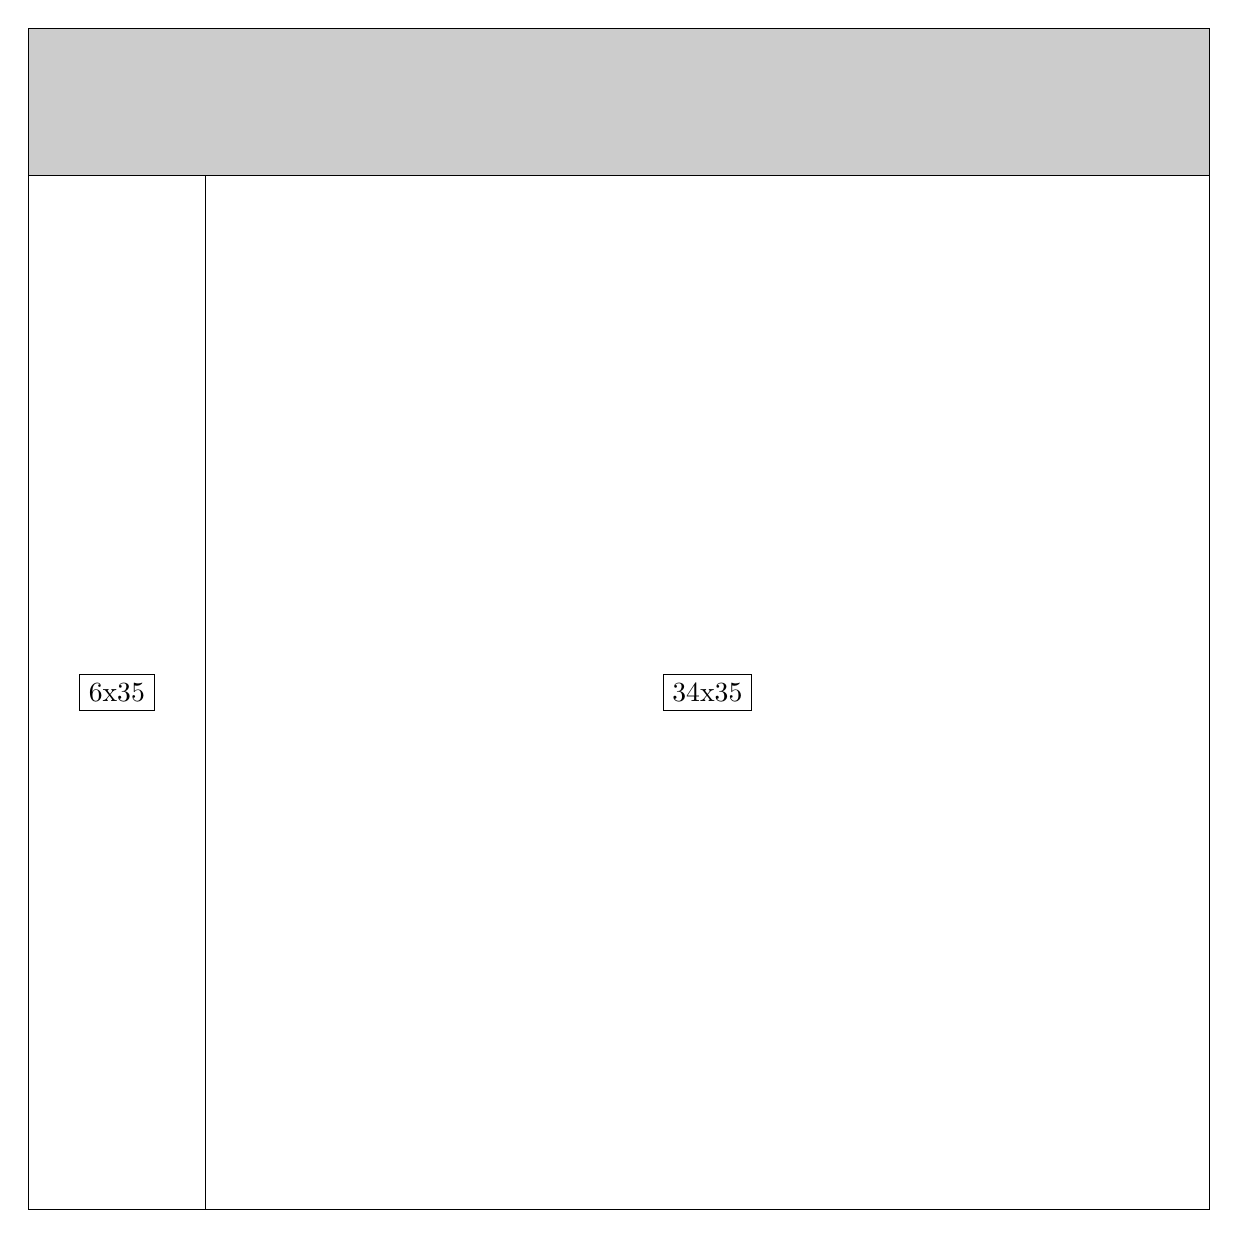
\begin{tikzpicture}[shorten >=1pt,scale=1.0,every node/.style={scale=1.0},->]
\tikzstyle{vertex}=[circle,fill=black!25,minimum size=14pt,inner sep=0pt]
\filldraw[fill=gray!40!white, draw=black] (0,0) rectangle (15.0,15.0);
\foreach \name/\x/\y/\w/\h in {34x35/2.25/0.0/12.75/13.125,6x35/0.0/0.0/2.25/13.125}
\filldraw[fill=white!40!white, draw=black] (\x,\y) rectangle node[draw] (\name) {\name} ++(\w,\h);
\end{tikzpicture}


w =34 , h =35 , x =6 , y =0 , v =1190
\par
w =6 , h =35 , x =0 , y =0 , v =210
\par
\newpage


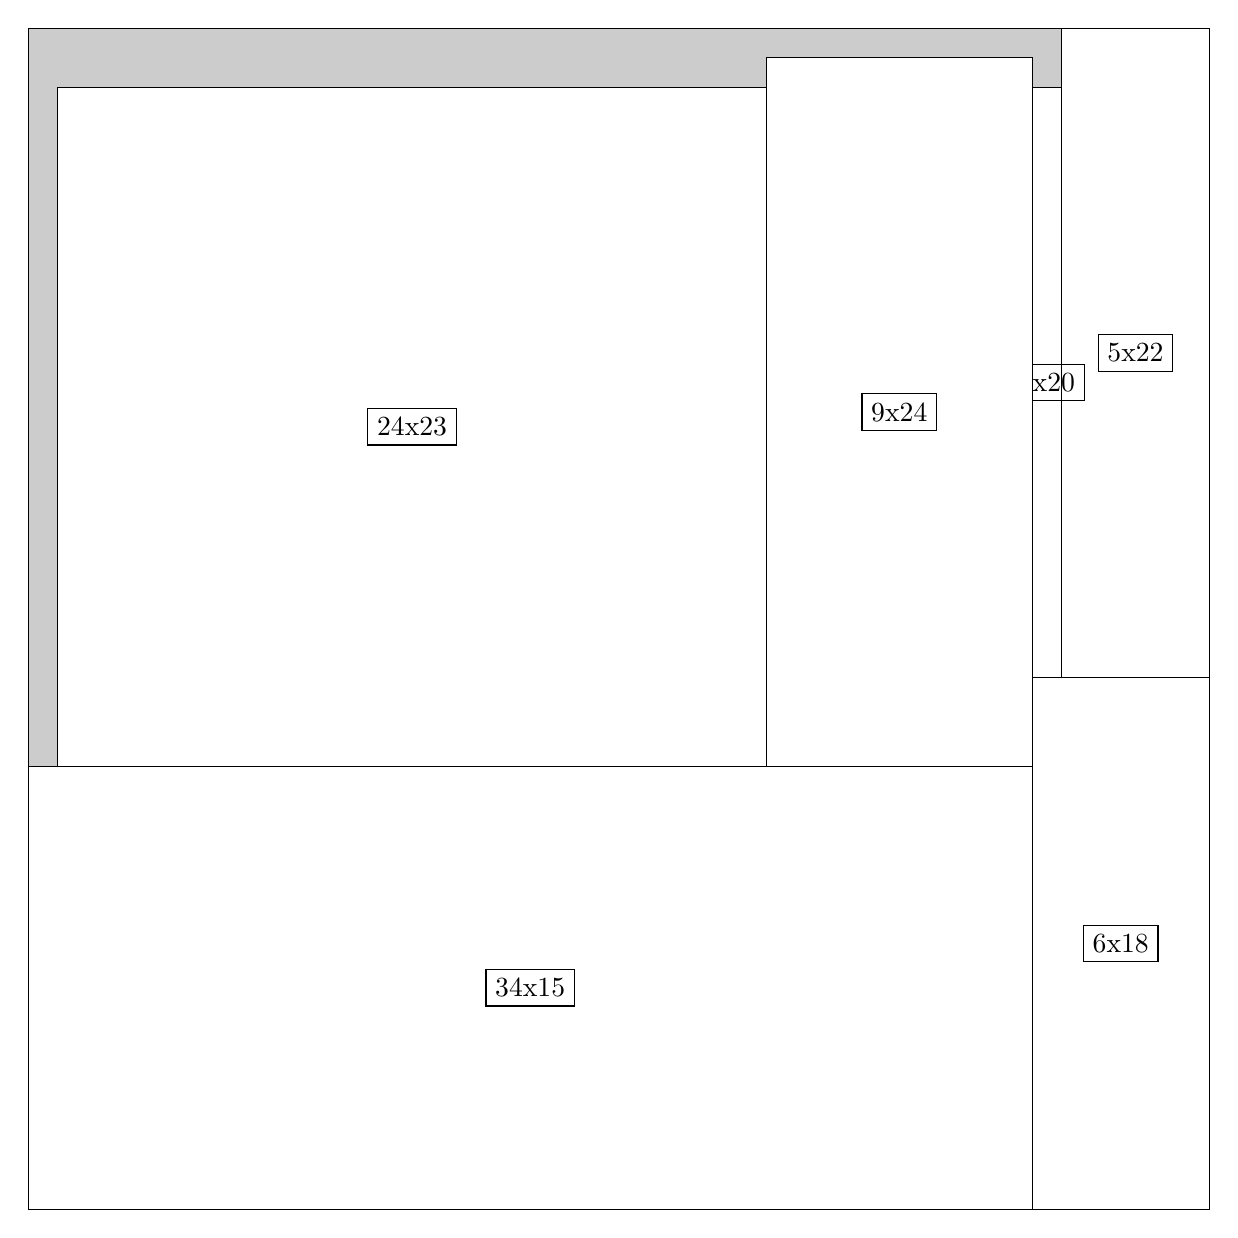
\begin{tikzpicture}[shorten >=1pt,scale=1.0,every node/.style={scale=1.0},->]
\tikzstyle{vertex}=[circle,fill=black!25,minimum size=14pt,inner sep=0pt]
\filldraw[fill=gray!40!white, draw=black] (0,0) rectangle (15.0,15.0);
\foreach \name/\x/\y/\w/\h in {6x18/12.75/0.0/2.25/6.75,5x22/13.125/6.75/1.875/8.25,1x20/12.75/6.75/0.375/7.5,34x15/0.0/0.0/12.75/5.625,9x24/9.375/5.625/3.375/9.0,24x23/0.375/5.625/9.0/8.625}
\filldraw[fill=white!40!white, draw=black] (\x,\y) rectangle node[draw] (\name) {\name} ++(\w,\h);
\end{tikzpicture}


w =6 , h =18 , x =34 , y =0 , v =108
\par
w =5 , h =22 , x =35 , y =18 , v =110
\par
w =1 , h =20 , x =34 , y =18 , v =20
\par
w =34 , h =15 , x =0 , y =0 , v =510
\par
w =9 , h =24 , x =25 , y =15 , v =216
\par
w =24 , h =23 , x =1 , y =15 , v =552
\par
\newpage


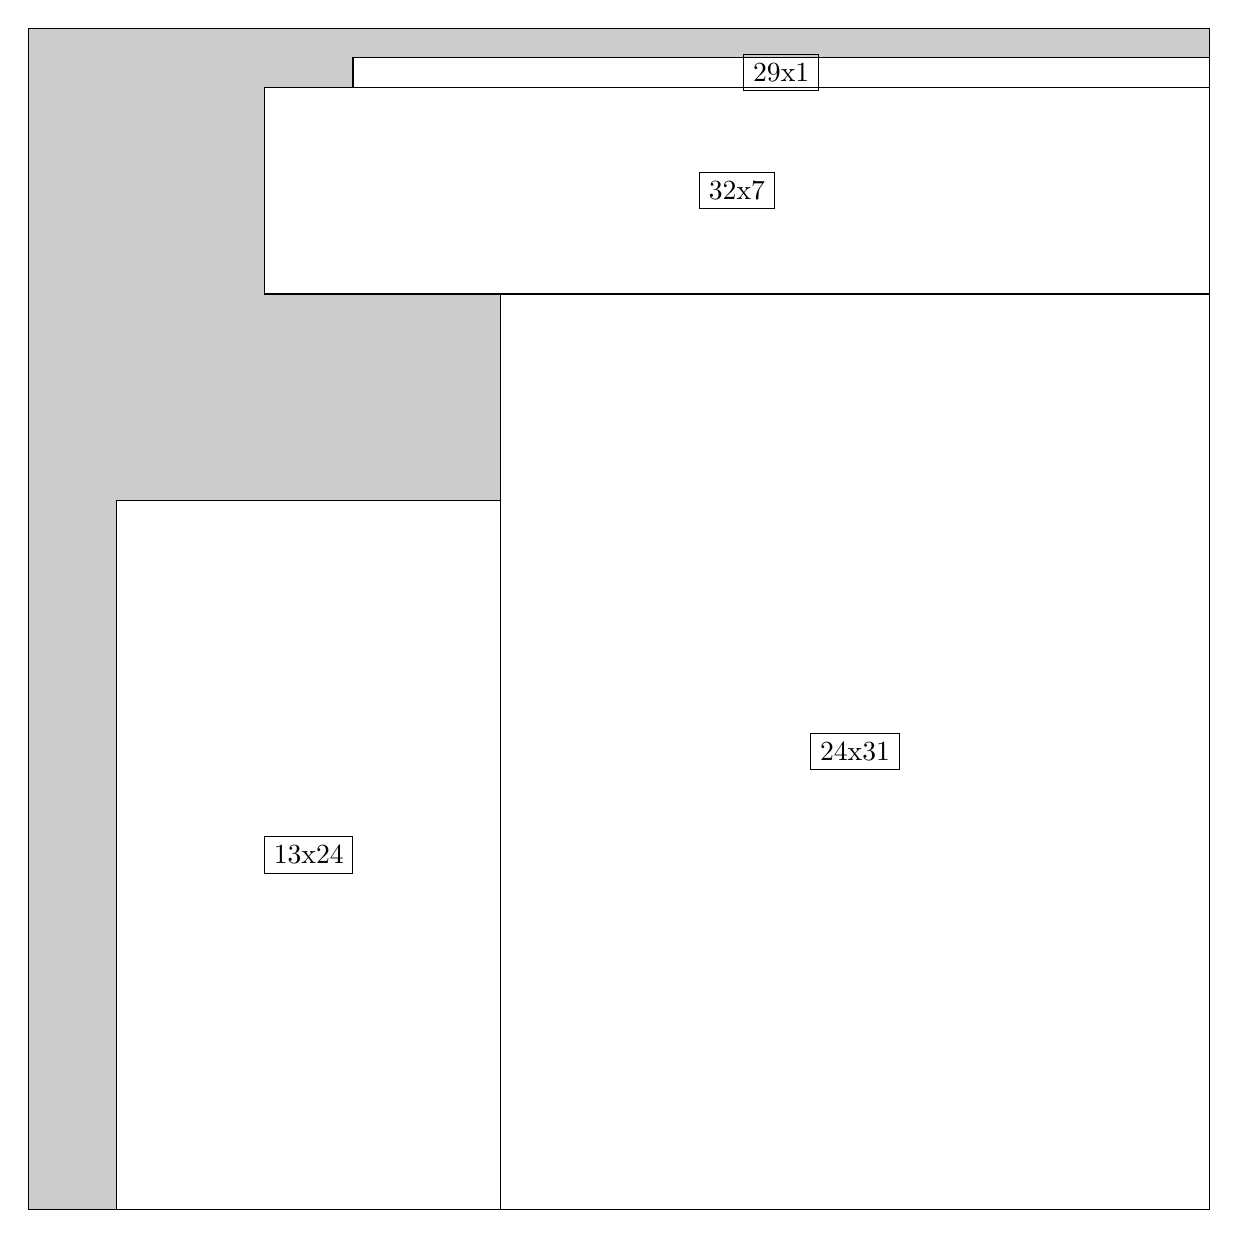
\begin{tikzpicture}[shorten >=1pt,scale=1.0,every node/.style={scale=1.0},->]
\tikzstyle{vertex}=[circle,fill=black!25,minimum size=14pt,inner sep=0pt]
\filldraw[fill=gray!40!white, draw=black] (0,0) rectangle (15.0,15.0);
\foreach \name/\x/\y/\w/\h in {24x31/6.0/0.0/9.0/11.625,13x24/1.125/0.0/4.875/9.0,32x7/3.0/11.625/12.0/2.625,29x1/4.125/14.25/10.875/0.375}
\filldraw[fill=white!40!white, draw=black] (\x,\y) rectangle node[draw] (\name) {\name} ++(\w,\h);
\end{tikzpicture}


w =24 , h =31 , x =16 , y =0 , v =744
\par
w =13 , h =24 , x =3 , y =0 , v =312
\par
w =32 , h =7 , x =8 , y =31 , v =224
\par
w =29 , h =1 , x =11 , y =38 , v =29
\par
\newpage


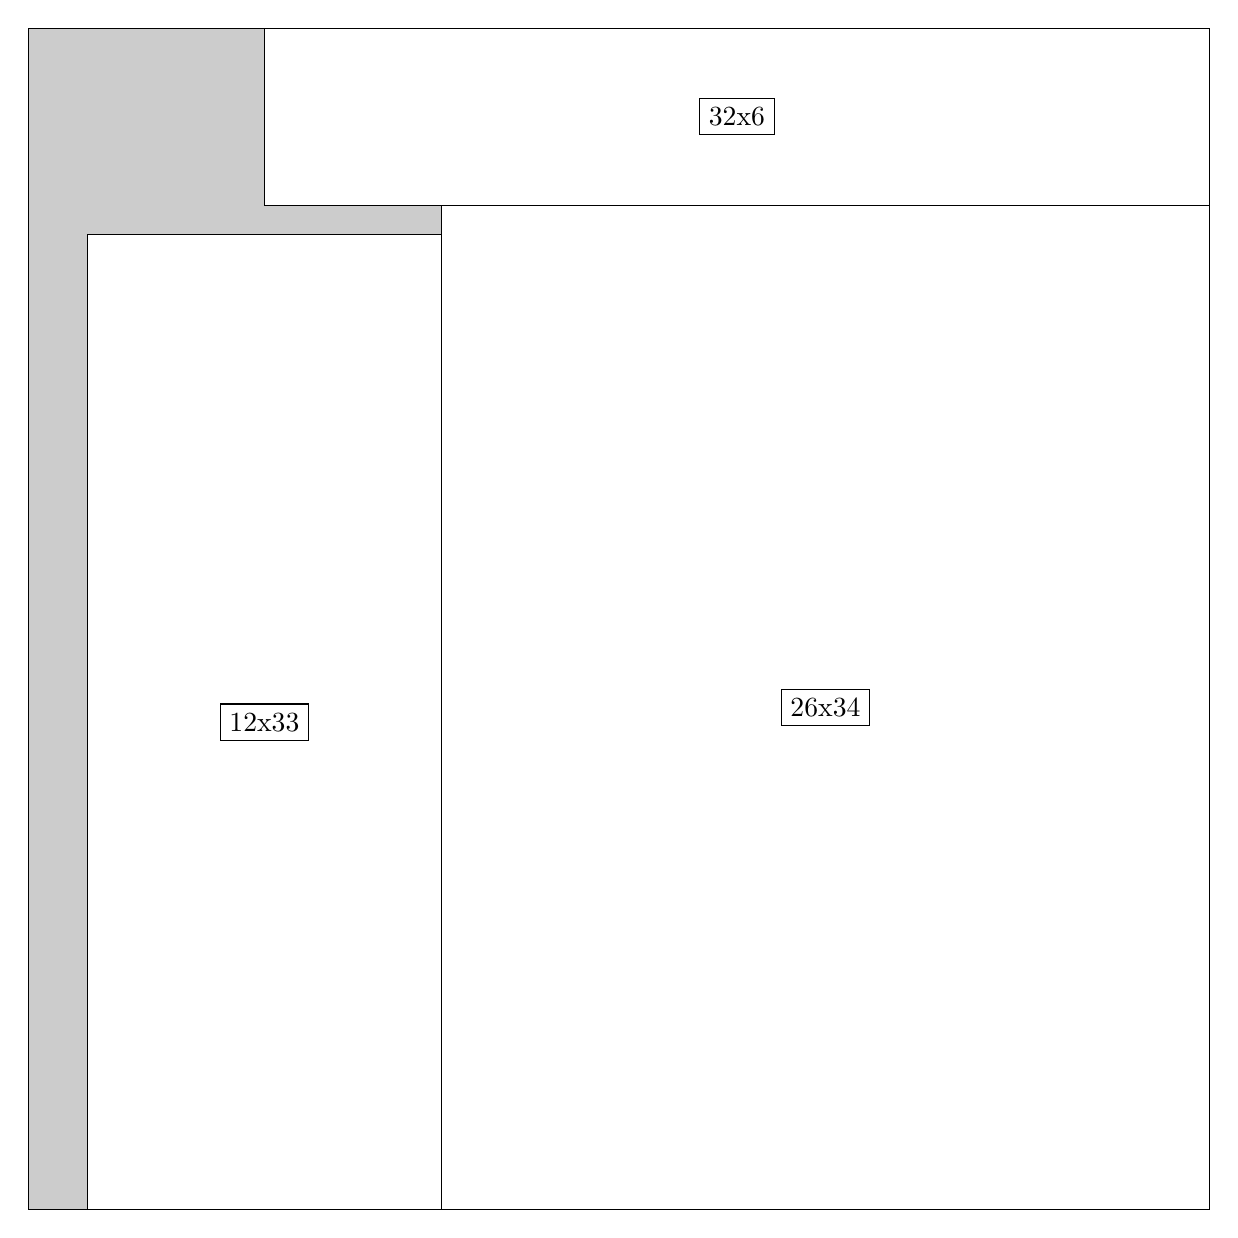
\begin{tikzpicture}[shorten >=1pt,scale=1.0,every node/.style={scale=1.0},->]
\tikzstyle{vertex}=[circle,fill=black!25,minimum size=14pt,inner sep=0pt]
\filldraw[fill=gray!40!white, draw=black] (0,0) rectangle (15.0,15.0);
\foreach \name/\x/\y/\w/\h in {26x34/5.25/0.0/9.75/12.75,12x33/0.75/0.0/4.5/12.375,32x6/3.0/12.75/12.0/2.25}
\filldraw[fill=white!40!white, draw=black] (\x,\y) rectangle node[draw] (\name) {\name} ++(\w,\h);
\end{tikzpicture}


w =26 , h =34 , x =14 , y =0 , v =884
\par
w =12 , h =33 , x =2 , y =0 , v =396
\par
w =32 , h =6 , x =8 , y =34 , v =192
\par
\newpage


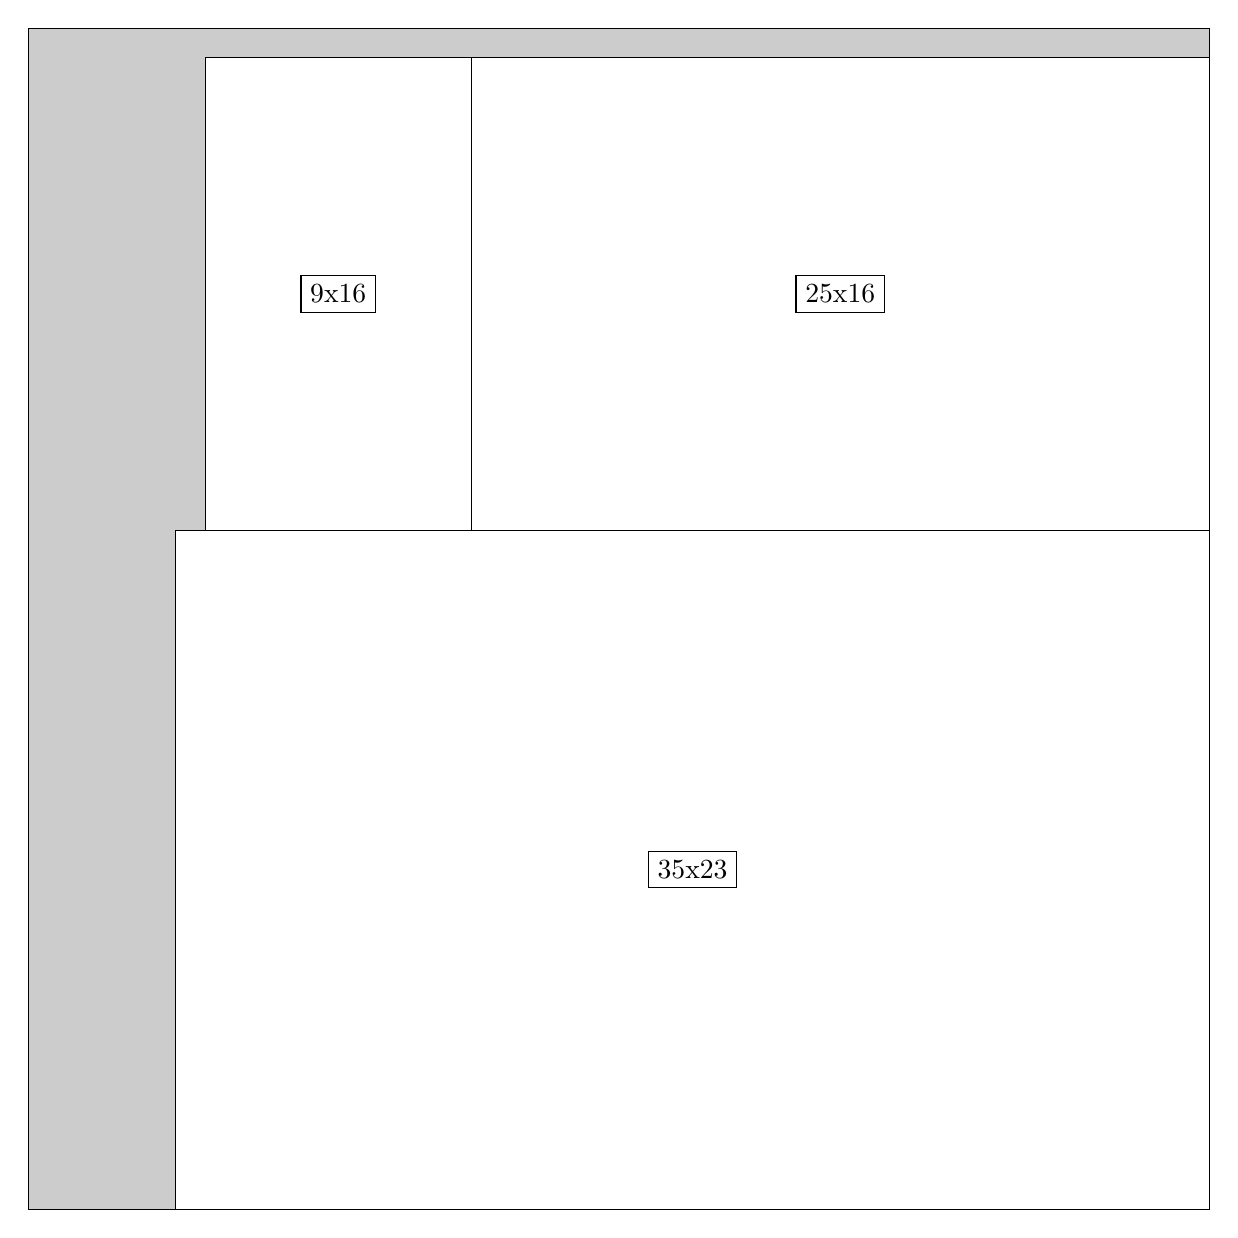
\begin{tikzpicture}[shorten >=1pt,scale=1.0,every node/.style={scale=1.0},->]
\tikzstyle{vertex}=[circle,fill=black!25,minimum size=14pt,inner sep=0pt]
\filldraw[fill=gray!40!white, draw=black] (0,0) rectangle (15.0,15.0);
\foreach \name/\x/\y/\w/\h in {35x23/1.875/0.0/13.125/8.625,25x16/5.625/8.625/9.375/6.0,9x16/2.25/8.625/3.375/6.0}
\filldraw[fill=white!40!white, draw=black] (\x,\y) rectangle node[draw] (\name) {\name} ++(\w,\h);
\end{tikzpicture}


w =35 , h =23 , x =5 , y =0 , v =805
\par
w =25 , h =16 , x =15 , y =23 , v =400
\par
w =9 , h =16 , x =6 , y =23 , v =144
\par
\newpage


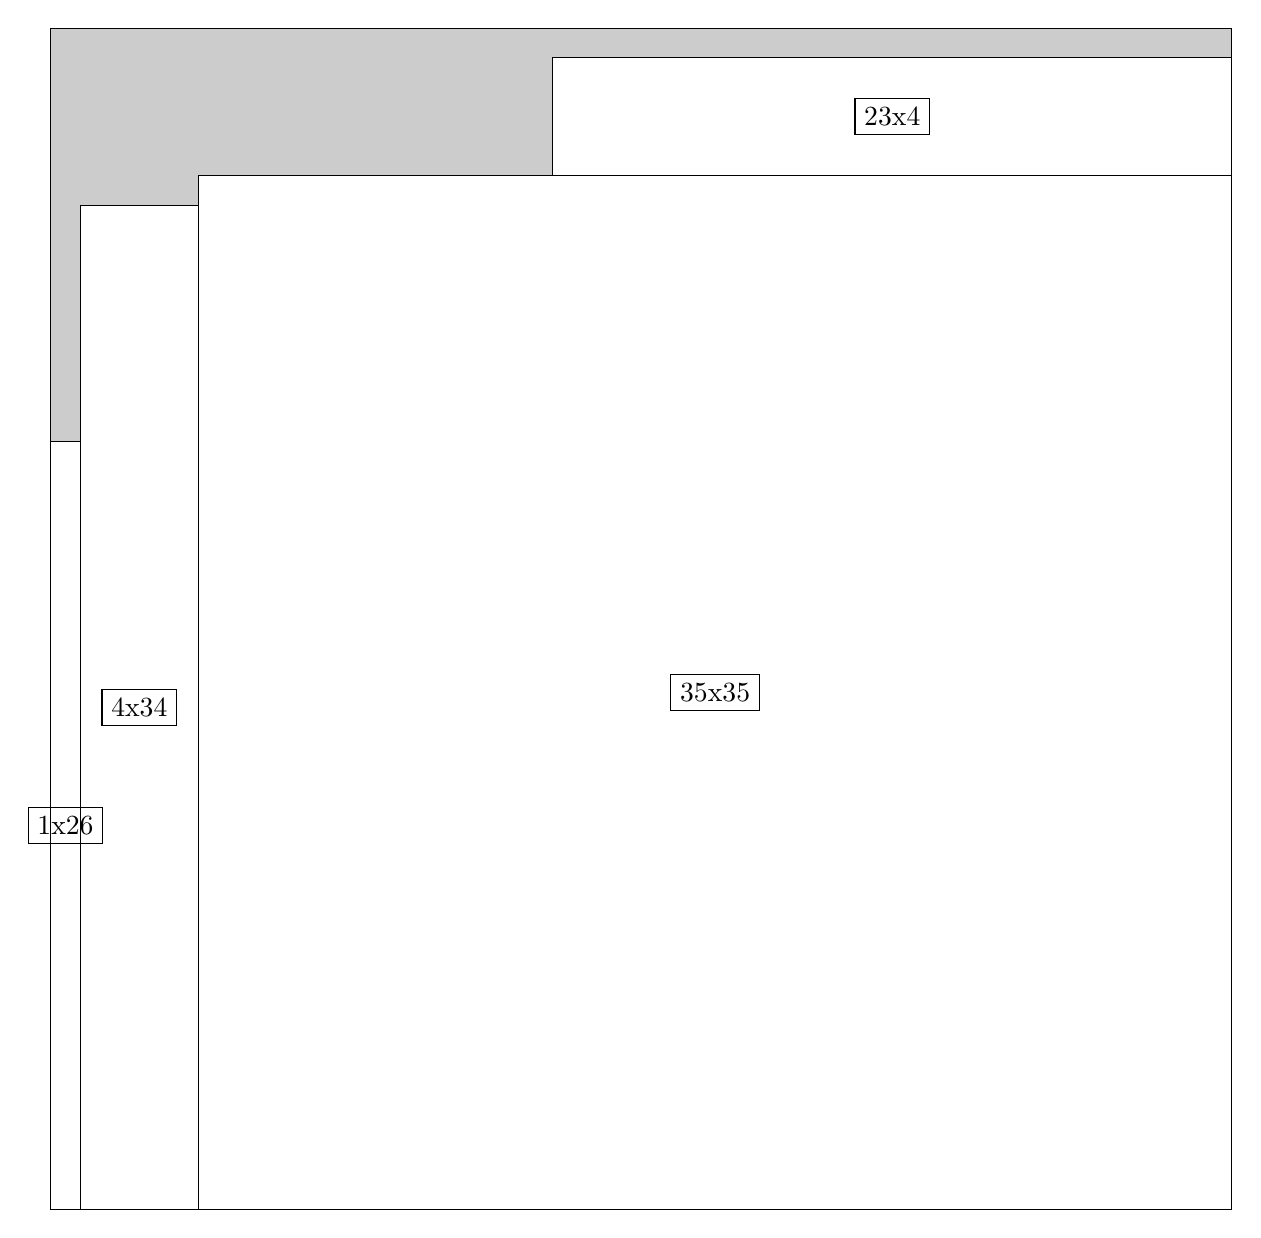
\begin{tikzpicture}[shorten >=1pt,scale=1.0,every node/.style={scale=1.0},->]
\tikzstyle{vertex}=[circle,fill=black!25,minimum size=14pt,inner sep=0pt]
\filldraw[fill=gray!40!white, draw=black] (0,0) rectangle (15.0,15.0);
\foreach \name/\x/\y/\w/\h in {35x35/1.875/0.0/13.125/13.125,4x34/0.375/0.0/1.5/12.75,1x26/0.0/0.0/0.375/9.75,23x4/6.375/13.125/8.625/1.5}
\filldraw[fill=white!40!white, draw=black] (\x,\y) rectangle node[draw] (\name) {\name} ++(\w,\h);
\end{tikzpicture}


w =35 , h =35 , x =5 , y =0 , v =1225
\par
w =4 , h =34 , x =1 , y =0 , v =136
\par
w =1 , h =26 , x =0 , y =0 , v =26
\par
w =23 , h =4 , x =17 , y =35 , v =92
\par
\newpage


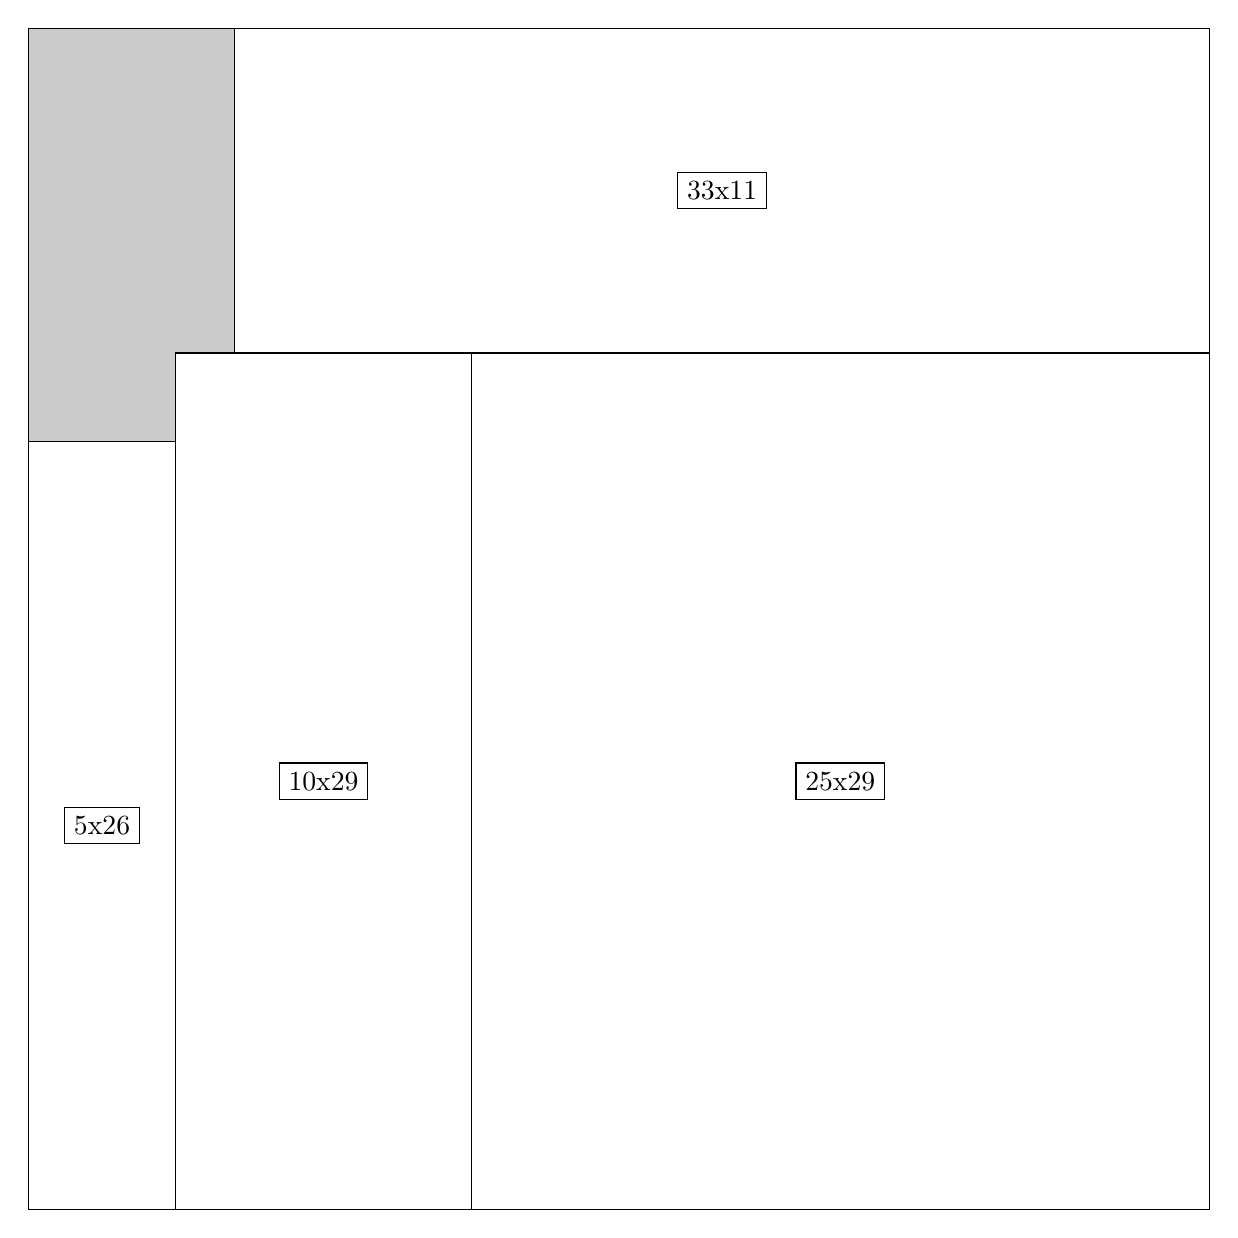
\begin{tikzpicture}[shorten >=1pt,scale=1.0,every node/.style={scale=1.0},->]
\tikzstyle{vertex}=[circle,fill=black!25,minimum size=14pt,inner sep=0pt]
\filldraw[fill=gray!40!white, draw=black] (0,0) rectangle (15.0,15.0);
\foreach \name/\x/\y/\w/\h in {25x29/5.625/0.0/9.375/10.875,10x29/1.875/0.0/3.75/10.875,5x26/0.0/0.0/1.875/9.75,33x11/2.625/10.875/12.375/4.125}
\filldraw[fill=white!40!white, draw=black] (\x,\y) rectangle node[draw] (\name) {\name} ++(\w,\h);
\end{tikzpicture}


w =25 , h =29 , x =15 , y =0 , v =725
\par
w =10 , h =29 , x =5 , y =0 , v =290
\par
w =5 , h =26 , x =0 , y =0 , v =130
\par
w =33 , h =11 , x =7 , y =29 , v =363
\par
\newpage


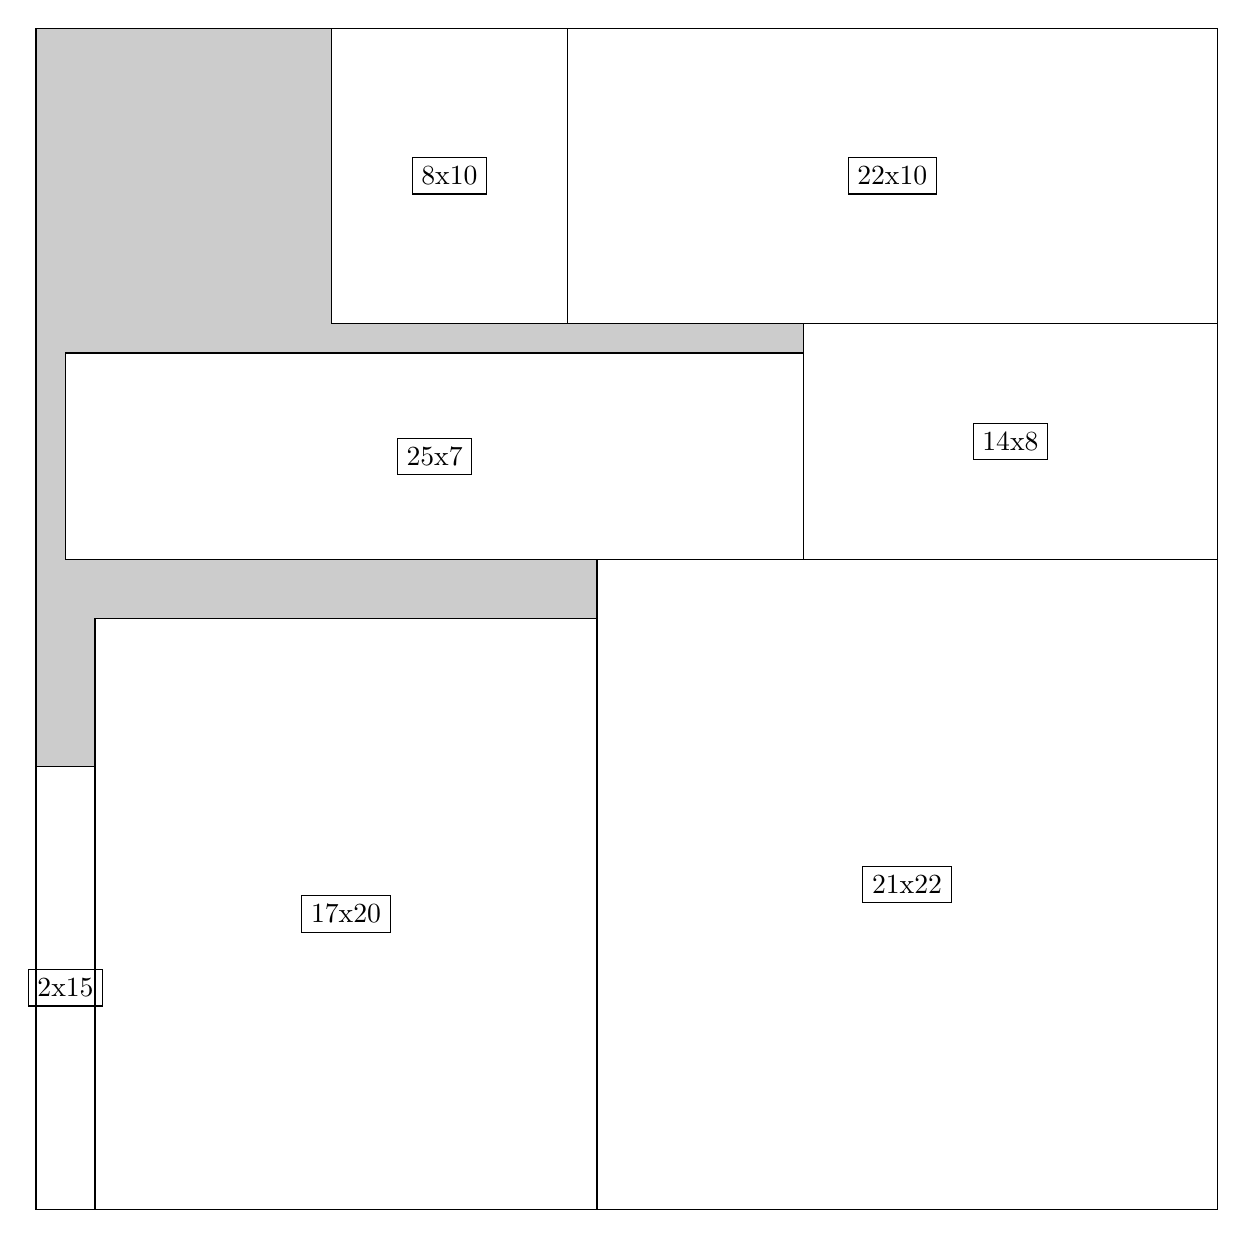
\begin{tikzpicture}[shorten >=1pt,scale=1.0,every node/.style={scale=1.0},->]
\tikzstyle{vertex}=[circle,fill=black!25,minimum size=14pt,inner sep=0pt]
\filldraw[fill=gray!40!white, draw=black] (0,0) rectangle (15.0,15.0);
\foreach \name/\x/\y/\w/\h in {21x22/7.125/0.0/7.875/8.25,17x20/0.75/0.0/6.375/7.5,2x15/0.0/0.0/0.75/5.625,14x8/9.75/8.25/5.25/3.0,25x7/0.375/8.25/9.375/2.625,22x10/6.75/11.25/8.25/3.75,8x10/3.75/11.25/3.0/3.75}
\filldraw[fill=white!40!white, draw=black] (\x,\y) rectangle node[draw] (\name) {\name} ++(\w,\h);
\end{tikzpicture}


w =21 , h =22 , x =19 , y =0 , v =462
\par
w =17 , h =20 , x =2 , y =0 , v =340
\par
w =2 , h =15 , x =0 , y =0 , v =30
\par
w =14 , h =8 , x =26 , y =22 , v =112
\par
w =25 , h =7 , x =1 , y =22 , v =175
\par
w =22 , h =10 , x =18 , y =30 , v =220
\par
w =8 , h =10 , x =10 , y =30 , v =80
\par
\newpage


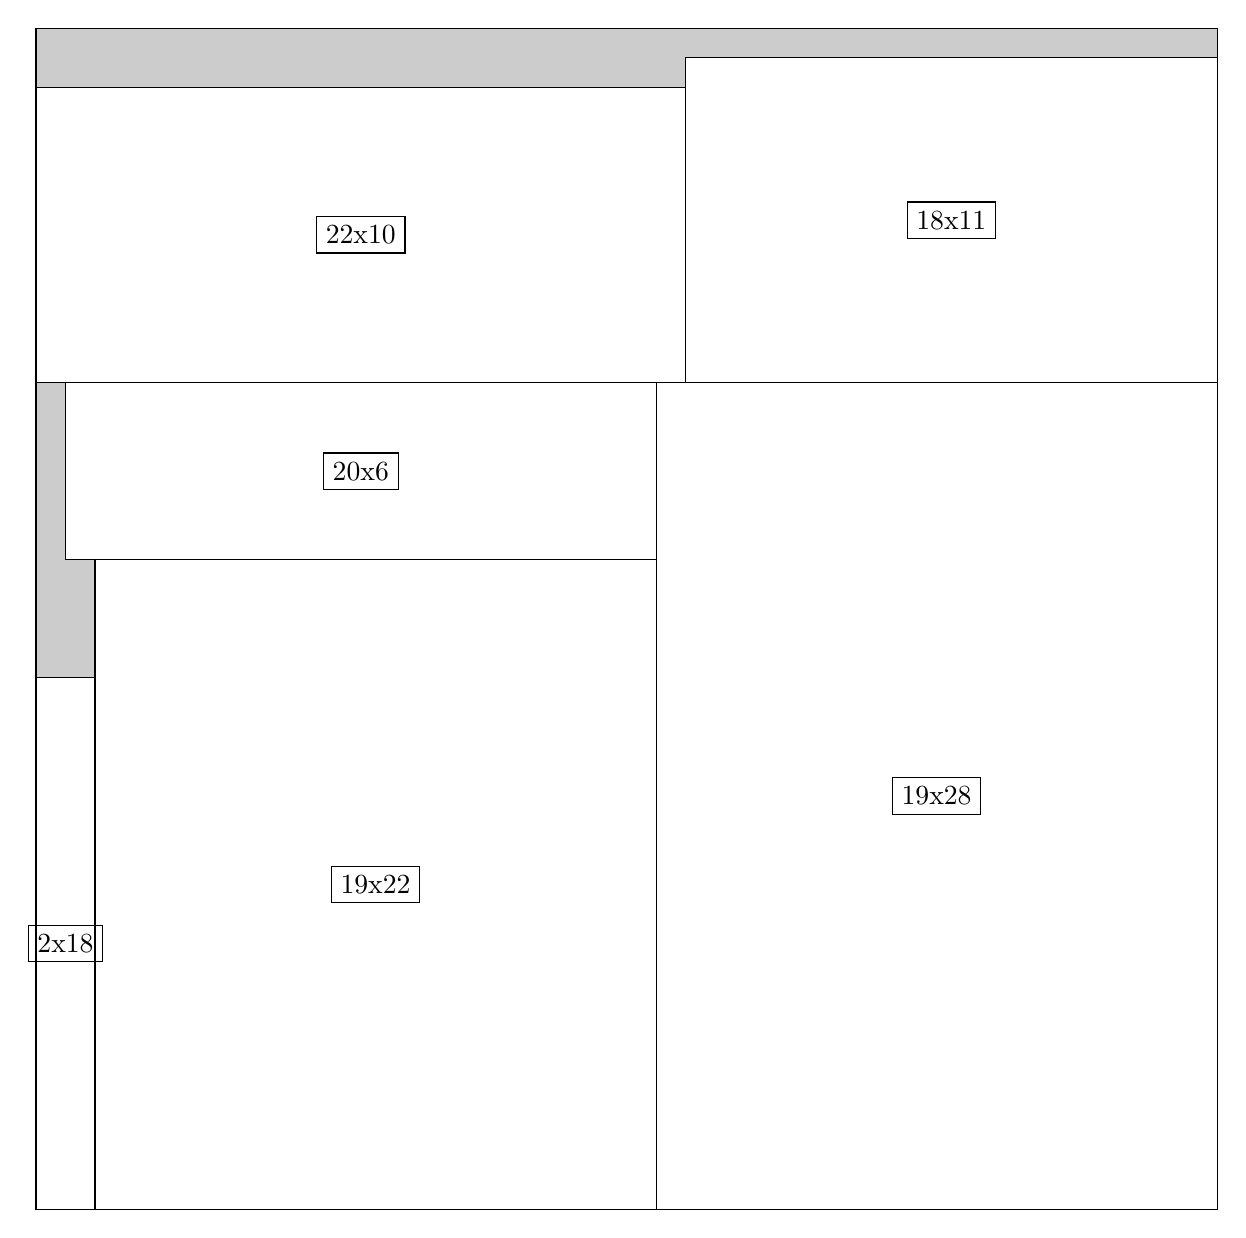
\begin{tikzpicture}[shorten >=1pt,scale=1.0,every node/.style={scale=1.0},->]
\tikzstyle{vertex}=[circle,fill=black!25,minimum size=14pt,inner sep=0pt]
\filldraw[fill=gray!40!white, draw=black] (0,0) rectangle (15.0,15.0);
\foreach \name/\x/\y/\w/\h in {19x28/7.875/0.0/7.125/10.5,19x22/0.75/0.0/7.125/8.25,2x18/0.0/0.0/0.75/6.75,20x6/0.375/8.25/7.5/2.25,18x11/8.25/10.5/6.75/4.125,22x10/0.0/10.5/8.25/3.75}
\filldraw[fill=white!40!white, draw=black] (\x,\y) rectangle node[draw] (\name) {\name} ++(\w,\h);
\end{tikzpicture}


w =19 , h =28 , x =21 , y =0 , v =532
\par
w =19 , h =22 , x =2 , y =0 , v =418
\par
w =2 , h =18 , x =0 , y =0 , v =36
\par
w =20 , h =6 , x =1 , y =22 , v =120
\par
w =18 , h =11 , x =22 , y =28 , v =198
\par
w =22 , h =10 , x =0 , y =28 , v =220
\par
\newpage


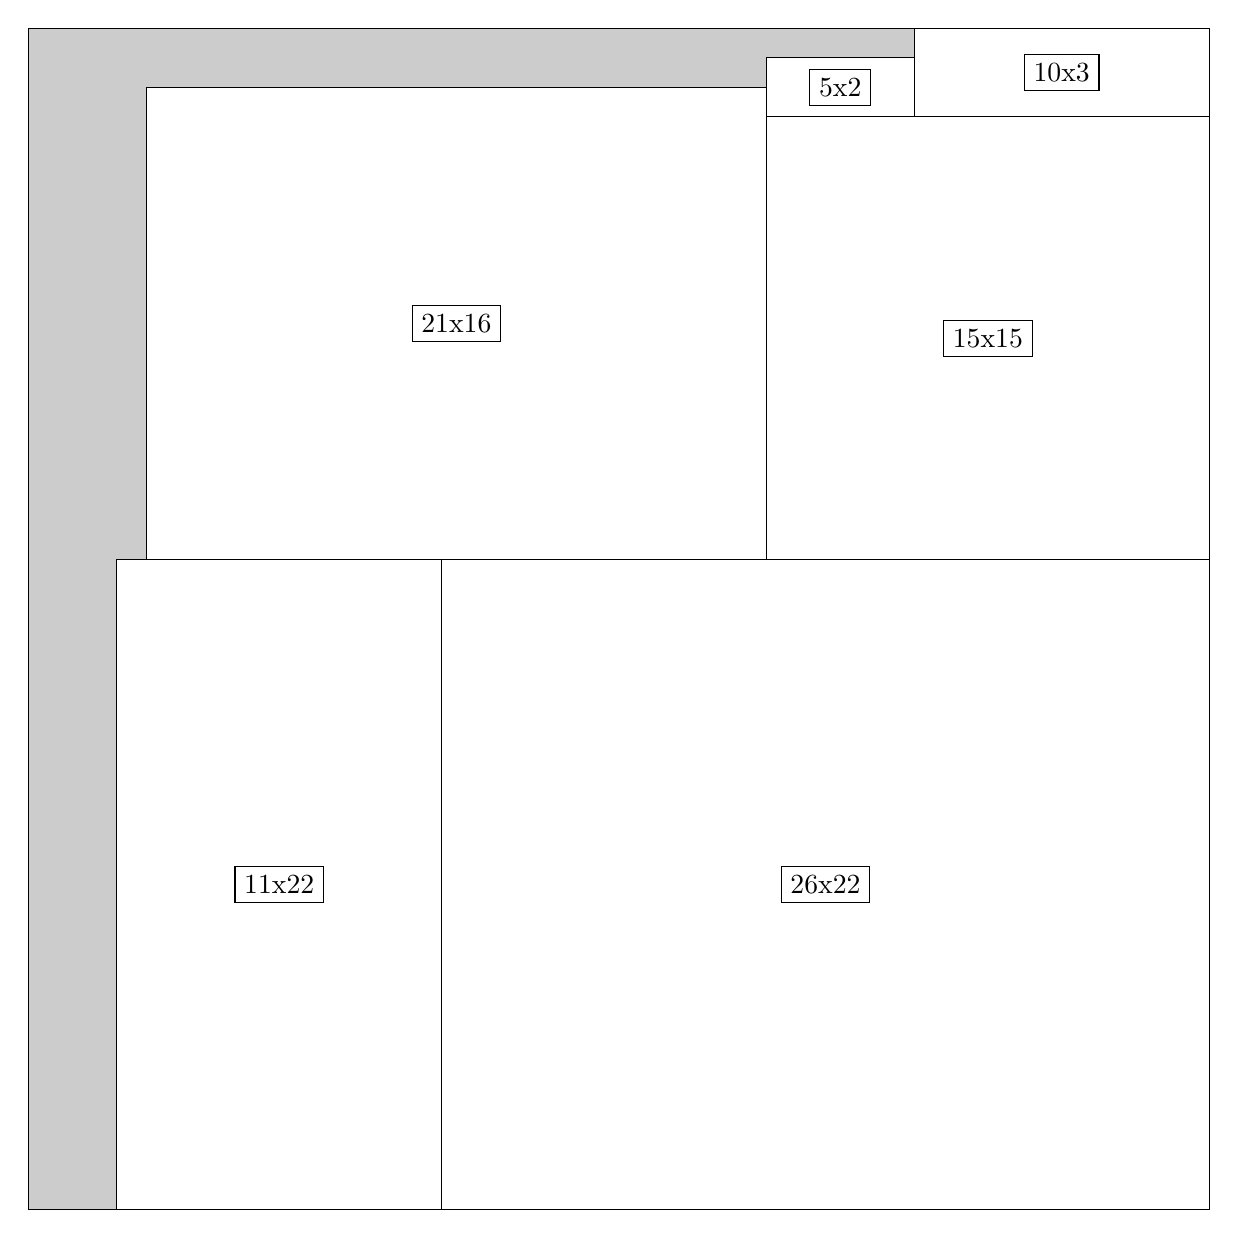
\begin{tikzpicture}[shorten >=1pt,scale=1.0,every node/.style={scale=1.0},->]
\tikzstyle{vertex}=[circle,fill=black!25,minimum size=14pt,inner sep=0pt]
\filldraw[fill=gray!40!white, draw=black] (0,0) rectangle (15.0,15.0);
\foreach \name/\x/\y/\w/\h in {26x22/5.25/0.0/9.75/8.25,11x22/1.125/0.0/4.125/8.25,15x15/9.375/8.25/5.625/5.625,10x3/11.25/13.875/3.75/1.125,5x2/9.375/13.875/1.875/0.75,21x16/1.5/8.25/7.875/6.0}
\filldraw[fill=white!40!white, draw=black] (\x,\y) rectangle node[draw] (\name) {\name} ++(\w,\h);
\end{tikzpicture}


w =26 , h =22 , x =14 , y =0 , v =572
\par
w =11 , h =22 , x =3 , y =0 , v =242
\par
w =15 , h =15 , x =25 , y =22 , v =225
\par
w =10 , h =3 , x =30 , y =37 , v =30
\par
w =5 , h =2 , x =25 , y =37 , v =10
\par
w =21 , h =16 , x =4 , y =22 , v =336
\par
\newpage


\end{document}